\chapter{Greedy}
Per illustrare il progetto e l'analisi di un algoritmo greedy consideriamo qualche problema.

\section{Algoritmi greedy}
\subsection{Selezione di attività}
    \textit{Abbiamo una lista di $n$ attività da eseguire: ciascuna attività è caratterizzata da una coppia con il suo tempo di inizio ed il suo tempo di fine, due attività sono compatibili se non si sovrappongono. Vogliamo trovare un sottoinsieme di attività compatibili di massima cardinalità.}

    \begin{figure}[ht]
    \centering
    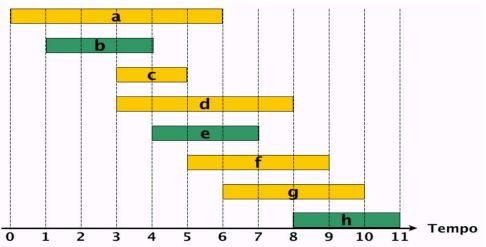
\includegraphics[width=0.6\linewidth]{images/es-selezione-attivita.JPG}
    \caption{Istanza del problema con n = 8}
    \label{fig:es-selezione-attiva}
    \end{figure}

    Volendo utilizzare il paradigma greedy dovremmo trovare una regola, semplice da calcolare, che ci permetta di effettuare ogni volta la scelta giusta. Per questo problema ci sono diverse potenziali regole di scelta: prendi l'attività compatibile che inizia prima;  prendi l'attività compatibile che dura meno; prendi l'attività compatibile che ha meno conflitti con le rimanenti.

    La regola giusta sta nel prendere sempre l'attività compatibile che finisce prima.

    \begin{demonstration}
        Supponiamo per assurdo che la soluzione greedy $SOL$ trovata con questa regola non sia ottima. Le soluzioni ottime differiscono dunque da $SOL$. Nel caso ci fossero più di una soluzione ottima prendiamo quella che differisce nel minor numero di attività da $SOL$, sia $SOL^*$. Dimostreremo ora che esiste un'altra soluzione ottima $SOL'$ che differisce ancora meno da $SOL$ il che è assurdo.

        Siano $A1, A2, ...$ le attività nell'ordine in cui sono state selezionate dal greedy sia $A_i$ la prima attività scelta dal greedy e non dall'ottimo (questa attività deve esistere perché tutte le attività scartate dal greedy erano incompatibili con quelle prese dal greedy e se la soluzione avesse preso tutte le attività scelte dal greedy non potrebbe averne prese di più). Nell'ottimo deve esserci un'altra attività $A'$ che va in conflitto con $A_i$ (altrimenti $SOL^*$ non sarebbe ottima in quanto potrei aggiungervi l'attività $A_i$). A questo punto posso sostituire in $SOL^*$ l'attività $A'$ con l'attività $A_i$ senza creare conflitti (perché in base alla regola di scelta greedy $A_i$ termina prima di $A'$). Ottengo in questo modo una soluzione ottima $SOL'$ (infatti le attività in $SOL'$ sono tutte compatibili e la cardinalità di $SOL'$ è la stessa di $SOL^*$). Ma $SOL'$ differisce da $SOL$ di un'attività in meno rispetto a $SOL^*$.
    \end{demonstration}

    Si può proseguire in questo modo:
    \begin{itemize}
        \item cercare in lista l'attività che finisce prima scorrendo la lista costerebbe $O(n)$ ad ogni iterazione del while. Conviene fare un pre-processing ordinando le attività in lista per tempo di fine crescente. In questo modo paghiamo $\Theta(n \log n)$ per l'ordinamento ma poi l'estrazione dell'attività ad ogni iterazione del file costerà $\Theta(1)$.
        \item Per eseguire efficientemente il test richiesto dall'if conviene mantenere una variabile con il tempo di fine dell'ultima attività inserita in soluzione in questo modo il test richiederà $\Theta(1)$.
    \end{itemize}

    L'algoritmo risultante è:
    \begin{lstlisting}[language=Python]
    def selezione_a(lista):
        lista.sort(key=lambda x:x[1])
        libero=0
        sol=[]
        for inizio, fine in lista:
            if libero<inizio:
                sol.append((inizio, fine))
                libero=fine
        return sol
    \end{lstlisting}
    Ordinare la lista delle attività costa $\Theta(n\log n)$. Il for viene eseguito $n$ volte e il costo di ogni iterazione è costante. Il costo finale è $\Theta(n\log n)$.

\subsection{Assegnazione di attività}
    \textit{Abbiamo una lista di attività, ciascuna caratterizzata da un tempo di inizio ed un tempo di fine. Le attività vanno tutte eseguite e vogliamo assegnarle al minor numero di aule tenendo conto che in una stessa aula non possono eseguirsi più attività in parallelo.}

    \begin{figure}[ht]
    \centering
    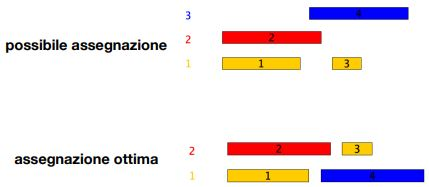
\includegraphics[width=0.6\textwidth]{images/es-assegnazione-attivita.JPG}
    \caption{Istanza del problema con \texttt{lista=[(1,4), (1,6), (7,8), (5,10)]}}
    \label{fig:es-assegnazione-attiva}
    \end{figure}

    Un possibile algoritmo greedy si basa sull'idea di occupare aule finché ci sono attività da assegnare e ad ogni aula, una volta inaugurata, assegnare il maggior numero di attività non ancora assegnate che è in grado di contenere.

    \begin{demonstration}
        Sia $k$ il numero di aule utilizzate dalla soluzione. Faremo vedere che ci sono nella lista $k$ attività incompatibili a coppie e questo ovviamente implica che $k$ aule sono necessarie.

        Sia $(a,b)$ l'attività che ha portato all'introduzione nella soluzione della $k$-ma aula. In quel momento nelle altre $k-1$ aule era impossibile eseguire l'attività $(a,b)$ ma per il criterio di scelta greedy posso anche dire che nell'istante di tempo $a$ erano tutte occupate (le attività loro assegnate iniziavano prima del tempo $a$ e non erano ancora finite) quindi nell'istante di tempo $a$ a due a due tutte queste $k$ attività sono incompatibili.
    \end{demonstration}

    Si può proseguire in questo modo:
    \begin{itemize}
        \item per individuare efficientemente l'attività che inizia prima effettuo un pre-processing in cui ordino le attività per tempo di inizio.
        \item per individuare efficientemente se una delle aule in soluzione è in grado di eseguire un certo lavoro $(a, b)$ uso un heap minimo in cui metto le coppie \verb|(libera, i)| dove $libera$ indica il tempo in cui si libera l'aula $i$. In questo modo in tempo $O(1)$ posso sapere qual'è l'aula che si libera prima semplicemente verificando \verb|H[0][0]|.

        Se nell'aula che si libera prima si può eseguire l'attività allora dovrò assegnargliela e aggiornare il valore $libera$ della coppia che la rappresenta nell'heap. Se al contrario l'aula non può accogliere l'attività allora non sarà possibile farlo in nessuna delle altre aule e bisognerà assegnare l'attività ad una nuova aula ed inserire nell'heap la coppia che rappresenta questa nuova aula.
    \end{itemize}
    
    L'algoritmo risultante è:
    \begin{lstlisting}[language=Python]
    def assegnazioneAule(lista):
        from heapq import heappop, heappush
        Sol=[[]]
        H=[(0,0)]
        lista.sort()
        for inizio, fine in lista:
            libera, aula = H[0]
            if libera<inizio:
                Sol[aula].append((inizio, fine))
                heappop(H)
                heappush(H, (fine, aula))
            else:
                Sol.append([(inizio, fine)])
                heappush(H, (fine, len(Sol)-1))
        return Sol
    \end{lstlisting}    
    Ordinare la lista costa $(n\log n)$, il for viene eseguito $n$ volte ed all'interno del for al caso pessimo può essere eseguita un'estrazione dall'heap seguita subito dopo da un inserimento nell'heap, entrambe operazioni di costo $O(\log n)$. Il for richiederà quindi tempo $O(n\log n)$. La complessità dell'algoritmo è $O(n\log n)$.

\subsection{File su disco}
    \textit{Abbiamo $n$ file di dimensioni $d_0, d_1,..., d_{n-1}$ che vorremmo memorizzare su un disco di capacità $k$. Tuttavia la somma delle dimensioni di questi file eccede la capacità del disco. Vogliamo dunque selezionare un sottoinsieme degli $n$ file che abbia cardinalità massima e che possa essere memorizzato sul disco. Descrivere un algoritmo greedy che risolve il problema in tempo $O(n\log n)$ e provarne la correttezza.}

    Ad esempio: per \verb|D=[5,6,3,5,4,7,3]| e \verb|k=11| la risposta deve essere la tripla di file 2, 4 e 6 che occupa spazio 10.

    Un algoritmo greedy per questo problema è quello che si presenta naturalmente: consideriamo i file per dimensione crescente e se c'è spazio per memorizzare il file su disco allora facciamolo.

    \begin{demonstration}
        Assumiamo per assurdo che la soluzione $sol$ prodotta dal greedy non sia ottima, devono quindi esistere insiemi con più file di $sol$ che rispettano la capacità del disco. Tra questi insiemi prendiamo quello con più elementi in comune con $sol$ e denotiamolo con $sol^*$. Nota che:
        \begin{itemize}
            \item esiste un file $a$ che appartiene a $sol^*$ e non a $sol$ e che occupa più spazio di qualunque file in $sol$ (questo perché tutti gli elementi in $sol$ occupano meno spazio di quelli non presenti in $sol$);
            \item esiste un file $b$ che appartiene a $sol$ e non a $sol^*$ (questo perché sol $sol\not\subset sol^*$ infatti l'aggiunta di un qualunque elemento a $sol$ porterebbe a superare la capacità del disco).
        \end{itemize}
        Posso dunque eliminare da $sol^*$ il file $a$ e inserire il file $b$ ottenendo un nuovo insieme di file che rispetta ancora le capacità del disco ed ha un elemento in più in comune con $sol$ contraddicendo la nostre ipotesi (il file $sol^*$ è quello con più elementi in comune con $sol$).
    \end{demonstration}

    L'algoritmo risultante è:
    \begin{lstlisting}[language=Python]
    def file(D, k):
        n = len(D)
        lista= [(D[i], i) for i in range(n)]
        lista.sort()
        spazio, sol = 0, []
        for d, i in lista:
            if spazio+d<=k:
                sol.append(i)
                spazio+=d
            else:
                return sol
    \end{lstlisting}
    La complessità dell'algoritmo è $\Theta(n \log n)$.

\subsection{Elementi in una lista}
    \textit{Abbiamo due liste di interi $A$ e $B$ ciascuna con $2n$ elementi. Dobbiamo selezionare $n$ elementi dalla lista $A$ ed $n$ elementi dalla lista $B$ in modo che la somma dei $2n$ elementi selezionati sia massima. Non è possibile selezionare elementi che nelle due liste occupino la stessa posizione. Progettare un algoritmo che prende come parametro le due liste $A$ e $B$ e in tempo $O(n\log n)$ restituisce la somma massima che si può ottenere. Motivare la correttezza e la complessità del vostro algoritmo.}

    Ad esempio: per \texttt{A = [10, 2, 4, 6, 1, 7, 3, 4]} e \texttt{B = [6, 6, 1, 0, 3, 8, 5, 7]} la selezione ottima si ottiene selezionando \texttt{A = [10, \_, 4, 6, \_, 7, \_, \_]} e \texttt{B = [\_, 6, \_, \_, 3, \_, 5, 7]}.

    La scelta di un elemento \verb|A[i]| significa anche perdere la possibilità di scegliere \verb|B[i]| quindi conviene massimizzare non tanto \verb|A[i]| quanto \verb|A[i] - B[i]|.

    Una implementazione diretta produrrebbe una complessità $O(n^{2})$ (infatti costerebbe $O(n)$ la ricerca dell'elemento $i$ per cui è massimo \verb|A[i] - B[i]|) e questa operazione andrebbe fatta $n$ volte all'interno del for. Per ottenere $O(n\log n)$ effettuo un pre-processing riordinando gli elementi di $A$ in modo che risulti decrescente il valore \verb|A[i] - B[i]|. Fatto questo ordinamento gli elementi da selezionare in $A$ saranno gli $n$ che risultano al primo posto della lista.

    \begin{demonstration}
        Sia $Sol^*$ il valore ottimo e $SOL$ il valore prodotto dall'algoritmo. Assumiamo per assurdo che $SOL$ e $Sol^*$ non coincidano e che quindi le scelte fatte dall'algoritmo e quelle che hanno portato a $Sol^*$ differiscono. Sia $Sol^*$ la sequenza di scelte che porta all'ottimo e che differisce meno dalle scelte fatte dall'algoritmo. Faremo vedere che esiste una sequenza di scelte $SOL'$ che porta all'ottimo e nelle scelte fatte differisce dall'algoritmo greedy meno di quanto faccia $Sol^*$.

        Sia $i$ un elemento in $A$ scelto dal greedy ma non in $Sol^*$ (un tale elemento deve esistere perché la soluzione ottima differisce dalla soluzione greedy). Deve anche esistere in $A$ un elemento $j$ preso dalla soluzione ottima ma non da quella greedy (perché entrambe le soluzioni pescano in ciascuno degli insiemi lo stesso numero di elementi). Deve aversi $A[i]-B[i] \geq A[j]-B[j]$ (grazie alla regola greedy che ha portato a scegliere l'elemento $i$ e non l'elemento $j$). Da cui deduciamo $A[i]-B[i]-A[j]+B[j]\geq 0$.

        Considera ora la soluzione $SOL'$ che si ottiene a partire da $Sol^*$ scambiando la scelta fatta per $i$ e $j$. Inserendo cioè gli elementi $i$ di $B$ al posto di quello di $A$ e l'elemento $j$ di $B$ al posto di quello di $A$. La soluzione $SOL'$ differisce meno da quella greedy di quanto faccia $Sol^*$. Resta da dimostrare che è ottima (vale ha dire che produce lo stesso valore di quella prodotta da $Sol^*$).

        La variazione di valore tra $SOL'$ e $Sol^*$ è data da $A[i]-B[i]-A[j]+B[j]$ e noi sappiamo che questo valore è positivo o nullo. Positivo non può essere (avremmo altrimenti trovato una soluzione che vale più dell'ottimo) deve quindi essere nulla. Questo significa che $SOL'$ e $Sol^*$ hanno lo stesso valore.
    \end{demonstration}

    L'algoritmo risultante è:
    \begin{lstlisting}[language=Python]
    def scelta(A, B):
        n=len(A)
        lista=[(A[i]-B[i], i) for i in range(n)]
        lista.sort(reverse=True)
        sol=0
        for i in range(n//2):
            sol+=A[lista[i][1]]
        for i in range(n//2, n):
            sol+=B[lista[i][1]]
        return sol
    \end{lstlisting}

    La complessità dell'algoritmo è $O(n \log n)$.

\section{Algoritmi di approssimazione}
Ci sono moltissimi problemi di ottimizzazione come la copertura tramite nodi che sono computazionalmente difficili. Per questi problemi non si conoscono algoritmi neanche lontanamente efficienti (sostanzialmente per questi problemi sono noti solo algoritmi esponenziali).

In questi casi potrebbe essere già soddisfacente ottenere una soluzione che sia soltanto "vicina" ad una soluzione ottima e, ovviamente, più è vicina e meglio è. Fra gli algoritmi che non trovano sempre una soluzione ottima, è importante distinguere due categorie piuttosto differenti: algoritmi di approssimazione ed euristiche.
\begin{itemize}
    \item Gli algoritmi di approssimazione sono algoritmi per cui si dimostra che la soluzione prodotta ha una certa "vicinanza" alla soluzione ottima. In altre parole, è garantito che la soluzione prodotta approssima entro un certo grado una soluzione ottima.
    \item Le euristiche sono algoritmi per cui non si riesce a dimostrare che la soluzione prodotta ha sempre una certa vicinanza ad una soluzione ottima. Però, sperimentalmente sembrano comportarsi bene. Sono l'ultima spiaggia, quando non si riesce a trovare algoritmi corretti efficienti né algoritmi di approssimazione efficienti che garantiscano un buon grado di approssimazione.
\end{itemize}
Per una gran parte dei problemi computazionalmente difficili non solo non si conoscono algoritmi corretti efficienti ma neanche buoni algoritmi di approssimazione. Non è quindi sorprendente che fra tutti i tipi di algoritmi, gli algoritmi euristici costituiscano la classe più ampia e che ha dato luogo ad una letteratura sterminata.

Un algoritmo di approssimazione per un dato problema è un algoritmo per cui si dimostra che la soluzione prodotta approssima sempre entro un certo grado una soluzione ottima per il problema. Si tratta quindi di specificare cosa si intende per "approssimazione entro un certo grado".

Iniziamo con problemi di minimizzazione (come ad esempio il problema della copertura tramite vertici) dove ad ogni soluzione ammissibile è associato un costo e cerchiamo quindi la soluzione ammissibile di costo minimo. Sia $p$ un qualsiasi problema di minimizzazione ed $I$ una sua istanza. Indichiamo con $OPT(I)$ il costo di una soluzione ottima per l'istanza e con $A(I)$ la soluzione prodotta dall'algoritmo $A$ per quell'istanza.

Il modo usuale di misurare il grado di approssimazione di un algoritmo di minimizzazione è il rapporto al caso pessimo tra il costo della soluzione prodotta dall'algoritmo e il costo della soluzione ottima: si dice che $A$ approssima $P$ entro un fattore di approssimazione $\rho$ se per ogni istanza $I$ di $P$ vale $\frac{A(I)}{OTT(I)}\leq\rho$.

Nota che risulta sempre $A(I) \geq OTT(I)$ di conseguenza il rapporto di approssimazione è sempre un numero maggiore o uguale ad 1.
\begin{itemize}
    \item Se $A$ approssima $P$ con fattore 1 allora $A$ è corretto per $P$ perché trova sempre una soluzione ottima.
    \item Se $A$ approssima $P$ entro un fattore 2 allora $A$ trova sempre una soluzione di costo al più doppio di quello della soluzione ottima.
    
    Ovviamente quanto più il rapporto d'approssimazione è vicino a 1 tanto più l'algoritmo d'approssimazione è buono.
\end{itemize}
Per problemi di massimizzazione dove ad ogni soluzione ammissibile è associato un valore si considera il rapporto inverso vale a dire $\frac{OTT(I)}{A(I)}$.

\subsection{Copertura tramite nodi minima}
    \textit{Dato un grafo non diretto $G$ una sua copertura tramite nodi è un sottoinsieme $S$ dei suoi nodi tale che tutti gli archi di $G$ hanno almeno un estremo in $S$. Dato un grafo non diretto $G$ trovare una copertura tramite nodi di minima cardinalità.}

    \begin{wrapfigure}{r}{0.30\textwidth}
        \vspace{-0.5cm}
        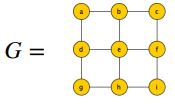
\includegraphics[width=0.28\textwidth]{images/es-copertura-tramite-nodi.JPG}
        \vspace{-0.5cm}
        %\caption{Birds}
    \end{wrapfigure}
    Una semplice strategia greedy per il problema potrebbe essere: finché ci sono archi non coperti inserisci in $S$ il nodo che copre il massimo numero di archi da coprire. Questo algoritmo non è corretto. Infatti sul grafo $G$ al primo passo verrebbe inserito in $S$ il nodo $e$ (l'unico a coprire 4 archi) dopodiché tutti i nodi restanti sono in grado di coprire lo stesso numero di archi e grado. La soluzione prodotta consiste di 5 nodi. Invece la soluzione ottima è formata dai 4 nodi $b$, $d$, $f$, $h$.

Proviamo a valutare il rapporto d'approssimazione dell'algoritmo greedy visto per il problema del copertura tramite nodi. L'algoritmo greedy che abbiamo proposto non è corretto (abbiamo trovato un'istanza per cui l'algoritmo produce una soluzione con 5 nodi mentre la soluzione ottima ha 4 nodi). Da ciò possiamo dedurre che il fattore di approssimazione dell'algoritmo è almeno $\frac{5}{4}>1$, ma potrebbe essere peggiore. In effetti per ogni costante $R$ si possono esibire grafi per cui l'algoritmo sbaglia di un fattore superiore ad $R$.

\begin{Lemma}{Rapporto di approssimazione $\Omega(\log l)$ per il copertura tramite nodi}{}
    Dimostreremo che per ogni intero $l$ possiamo costruire un grafo $G_l$ su cui l'algoritmo greedy avrà rapporto di approssimazione $\Omega(\log l)$.
    Il grafo $G_l$ è definito come segue: 
    \begin{itemize}
        \item il grafo è strutturato in $l$ livelli che vanno da 1 a $l$ e gli archi del grafo collegano nodi a livello $i > 1$ con nodi a livello 1. Più precisamente: a livello $i$ sono presenti $\frac{l}{i}$ nodi, ciascuno di questi nodi ha grado $i$ e gli $i\frac{l}{i}\leq l$ archi vanno a nodi distinti del livello 1.

        \begin{minipage}{\textwidth}
            \centering
            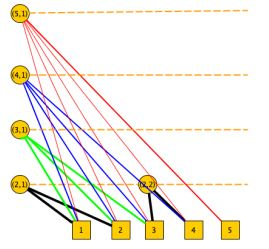
\includegraphics[width=0.4\textwidth]{images/rapp-appr-g5.JPG}
            \captionof{figure}{Esempio di grafo $G_5$}
        \end{minipage}
    \end{itemize}

    Sul grafo $G_l$ l'euristica funziona come segue: il primo nodo ad essere selezionato è il nodo a livello $l$ di grado $l$ (tutti gli altri hanno grado al più $l-1$); verranno poi uno dopo l'altro selezionati tutti i nodi a livello $l-1$ di grado $l-1$ (tutti gli altri hanno grado al più $l-2$); verranno poi uno dopo l'altro selezionati tutti i nodi a livello $l-2$ di grado $l-2$ (tutti gli altri hanno grado al più $l-3$) ... verranno infine selezionati tutti i nodi a livello $2$ di grado $2$ (tutti gli altri, cioè i nodi a livello $1$ hanno grado $1$).

    Per il costo della soluzione prodotta dall'euristica si ha:
    \begin{align*}
        c(SOL)=\sum^l_{i=2}\frac{l}{i}\geq\sum^l_{i=2}\left(\frac{l}{i}-1\right)\geq l\int^{l+1}_2\frac{1}{x}dx-(l-1)=l\log_e(l+1)-l\log_e2-l+1\geq\\\Omega(l\log l)
    \end{align*}

    Una possibile soluzione al problema è quella di selezionare gli $l$ nodi a livello 1 (infatti per costruzione tutti gli archi incidono su quegli $l$ nodi). Non è difficile dimostrare che questa è anche la soluzione ottima. Possiamo comunque dire $c(SOL)=O(l)$.

    Abbiamo quindi dimostrato che il rapporto di approssimazione dell'euristica è almeno $\frac{c(SOL)}{c(SOL*)}=\frac{\Omega(l\log l)}{O(l)}=\Omega(\log l)$.
\end{Lemma}

Ovviamente il fatto d'aver dimostrato che per un problema un certo algoritmo d'approssimazione ha un cattivo rapporto d'approssimazione non impedisce che per il problema possano esistere altri algoritmi d'approssimazione con un fattore d'approssimazione costante.

\begin{Algoritmo}{Algoritmo per la copertura dei nodi}{}
    Consideriamo il seguente algoritmo greedy per la copertura di nodi: considera i vari archi del grafo uno dopo l'altro e ogni volta che ne trovi uno non coperto (vale a dire nessuno dei suoi estremi è in $S$) aggiungi entrambi gli estremi dell'arco alla soluzione $S$.

    L'algoritmo produce ovviamente una copertura (ogni arco verrà infatti esaminato e se risulterà non coperto verrà coperto da entrambi i lati). La copertura prodotta non è detto sia minima, l'algoritmo ha rapporto d'approssimazione almeno 2 come dimostra il grafo con due soli nodi ed un arco. Dimostreremo che il rapporto d'approssimazione è limitato da 2.

    Per rendere efficiente il test sui nodi in $S$ utilizzo un vettore caratteristico \verb|presi| dove \verb|presi[i]=1| se il nodo $i$ è in $S$, 0 altrimenti.

    \begin{lstlisting}[language=Python]
    def copertura1(G):
        n=len(G)
        E=[(x, y) for x in range(n) for y in G[x] if x<y]
        presi=[0]*n
        Sol=[]
        for a, b in E:
            if presi[a]==presi[b]==0:
                Sol.append(a)
                Sol.append(b)
                presi[a]=presi[b]=1
        return Sol
    \end{lstlisting}

    \begin{minipage}{\textwidth}
        \centering
        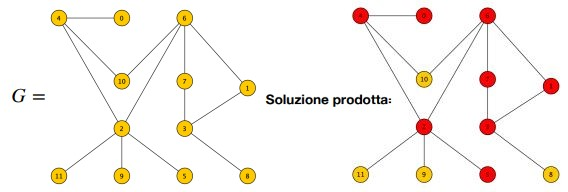
\includegraphics[width=0.9\textwidth]{images/alg-cop-nodi.JPG}
        %\captionof{figure}{Esempio di grafo $G_5$}
    \end{minipage}

    La complessità dell'algoritmo è $O(n+m)$.
\end{Algoritmo}

\begin{Lemma}{Il rapporto d'approssimazione dell'algoritmo greedy è limitato da 2}{}
    Siano $e_1, e_2, ... e_k$ gli archi di $G$ che vengono trovati non coperti durante l'esecuzione dell'algoritmo greedy.
    \begin{enumerate}
        \item Per come funziona l'algoritmo deduciamo che $A(I) = 2k$. 
        
        I $k$ archi non coperti sono tra loro disgiunti (infatti i due estremi di ciascuno di questi archi vengono incontrati per la prima volta quando viene esaminato l'arco) questo significa che in una qualunque delle soluzioni ottime almeno un estremo di ciascuno di questi $k$ archi deve essere presente.

        \item Ne deduciamo che $k\leq OTT(I)$.
    \end{enumerate}

    Dai punti 1) e 2) ricaviamo che $A(I) = 2k\leq 2*OTT(I)$ da cui segue $\frac{A(I)}{OTT(I)}\leq 2$.
\end{Lemma}

\subsection{Il problema del massimo taglio}
\textit{Dato un grafo $G$ non diretto e connesso un taglio di $G$ è un sottoinsieme $A$ dei suoi vertici. Il valore di un taglio è dato dal numero di archi che hanno esattamente un estremo in $A$. Vogliamo trovare il taglio di valore massimo.}

Si propone il seguente algoritmo greedy: parti con due insiemi $A$ e $B$ vuoti. Considera i vertici del grafo $G$ nell'ordine crescente e inseriscili in $A$ o $B$ in base alla regola che segue: ogni nodo $i$ può contribuire al taglio che si va via via creando apportando potenzialmente nuovi archi (quelli che incidono su di lui e sui nodi già considerati).
Sia $x$ il numero di questi archi. Inserisci $i$ in $A$ se così facendo il contributo al taglio è almeno $\frac{x}{2}$, inseriscilo in $B$ altrimenti. Dopo aver inserito ogni nodo nell'insieme opportuno restituisci $A$. 

Viene riportata una possibile implementazione di complessità $O(m)$:
\begin{lstlisting}[language=Python]
def MC(G): 
    n=len(G) 
    CA=[0]*n 
    CB=[0]*n
    A=[] 
    for i in range(n): 
        if CA[i] >= CB[i]: 
            A.append(i) 
            for u in G[i]: 
                if u>i: 
                    CB[u]+=1 
        else: 
            for u in G[i]:
                if u>i: 
                    CA[u]+=1
    return A
\end{lstlisting}
L'euristica ha un rapporto d'approssimazione limitato da 2.

Sia $k$ il valore della soluzione greedy e $k^*$ quello della soluzione ottima. Assegnamo la responsabilità di ciascun arco al suo estremo di indice massimo. Sia $r_i$ il numero di archi di cui il nodo $i$ è responsabile. Ovviamente vale
\begin{equation*}
    k^* \leq m = \sum^{n-1}_{i=0}r_i
\end{equation*}
Per la regola con cui viene assegnato il nodo $i$ ad $A$ o a $B$ si ha che il contributo di $i$ al taglio è almeno $\frac{r-i}{2}$. Quindi vale
\begin{equation*}
    \sum^{n-1}_{i=0}\frac{r_i}{2}\leq k
\end{equation*}
Dalle disequazioni 1) e 2) ricaviamo $k^* \leq \sum^{n-1}_{i=0}r_i=2\sum^{n-1}_{i=0}\frac{r_i}{2}\leq 2k$ e quindi $\frac{k^*}{k}\leq 2$.

Il rapporto d'approssimazione non può essere migliorato come mostra l'istanza con un grafo di $n$ nodi con i nodi 0 e 1 di grado $n - 1$ e tutti gli altri nodi di grado 2. L'euristica metterebbe il primo nodo in $A$ ed il secondo in $B$ a questo punto tutti i rimanenti nodi contribuirebbero al taglio per esattamente 1 (indipendentemente dall'insieme in cui vengono inseriti). Viene quindi prodotto un taglio di valore $n - 1$. Mettendo i primi due nodi del grafo in $A$ e tutti gli altri in $B$ si otterrebbe un taglio di valore $2(n - 2)$. Si ha quindi in questo caso
\begin{equation*}
    \frac{k^*}{k}\geq \frac{2(n-1)}{n-1}-\frac{2}{n-1}=2-\frac{2}{n-1}
\end{equation*}
che tende a 2 al crescere di $n$. Attualmente il miglior algoritmo approssimante per questo problema ha rapporto $\alpha \approx 1.389$.

\subsection{Il problema dell'impacchettamento (BP)}
\textit{Il problema dell'impacchettamento è un problema di ottimizzazione che consiste nell'impacchettare in scatole con capacità $c$ un insieme di $n$ oggetti ciascuno di dimensione intera al più $c$, minimizzando il numero di contenitori utilizzati.
Il problema richiede dunque di trovare la distribuzione degli oggetti all'interno
dei contenitori in modo da usare il minor numero possibile di contenitori, rispettando le dimensioni dei singoli oggetti e dei contenitori stessi.}

Il problema è notoriamente difficile e per ottenere soluzioni soddisfacenti in tempi ragionevoli si ricorre ad algoritmi di approssimazione. La più semplice euristica è di tipo greedy ed è nota come Next Fit, lavora come segue: si considerano gli oggetti da impacchettare in sequenza. All'inizio abbiamo un unico contenitore contenente il primo oggetto. Per ogni altro oggetto, se il contenitore ha spazio per contenerlo allora l'oggetto viene inserito nel contenitore, in caso contrario il contenitore viene chiuso e viene inaugurato un nuovo contenitore.

La procedura prende in input la lista dei pesi degli oggetti e la capacità delle scatole e restituisce il numero di scatole necessarie. La complessità è $\Theta(n)$:

\begin{lstlisting}[language=Python]
def NF(P, c):
    n=len(P)
    Sol=[[0]]
    spazio=c-P[0]
    for i in range (1, n):
        if spazio-P[i] >= 0:
            Sol[-1].append(i)
            spazio-=P[i]
        else:
            Sol.append([i])
            spazio=c-P[i]
    return len(Sol), Sol
\end{lstlisting}
L'euristica Next Fit ha un rapporto d'approssimazione limitato da 2.

Sia $k$ il numero di contenitori utilizzato dall'euristica e $k^*$ quello della soluzione ottima inoltre indichiamo con $s$ la somma delle dimensioni degli $n$ oggetti. Deve ovvviamente aversi

\begin{equation*}
    s\leq c*k^*
\end{equation*}
Nota che di due contenitori inaugurati in sequenza almeno uno è pieno per più della metà infatti se il primo dei due contenitori è pieno per meno della metà allora l'oggetto che ha portato all'inaugurazione del contenitore successivo deve avere una dimensione superiore alla metà di $c$. Questo significa che tutti i contenitori tranne l'ultimo sono pieni per più della metà. Abbiamo dunque

\begin{equation*}
    (k-1)\frac{c}{2}<s
\end{equation*}
Mettendo insieme le due diseguaglianze abbiamo $(k - 1)\frac{c}{2} < c * k^*$ da cui ricaviamo $k - 1 < 2k^*$ e, poiché $k$ e $k^*$ sono interi deve aversi $k \leq 2k^*$ da cui finalmente  deduciamo $\frac{k}{k^*}\leq 2$.

Il rapporto stabilito dal teorema non può essere migliorato come mostra la seguente istanza: considera una lista di $2c$ oggetti di peso $c$ e $2c$ oggetti di peso 1 da dover inserire
in scatole di dimensione $2c$. La soluzione ottima consiste nell'inserire due oggetti di dimensione $c$ in ciascuna scatola e poi utilizzare due scatole per inserire i $2c$ oggetti di dimensione 1. Il numero minimo di scatole $k^*$ necessarie è dunque $c + 2$ scatole. Tuttavia se nella lista gli oggetti delle due diverse dimensioni si alternano l'algoritmo NF utilizzerà $2c$ scatole inserendo in ogni scatola un oggetto di dimensione $c$ ed un oggetto di dimensione 1 producendo una soluzione che utilizza un numero di scatole $k$ pari a $2c$. Per questa istanza si ha dunque rapporto 

\begin{equation*}
    \frac{k}{k^*}=\frac{2c}{c+2}=\frac{2(c+2)}{c+2}-\frac{4}{c+2}=2-\frac{4}{c+2}
\end{equation*}
il rapporto al crescere di $c$ tende a 2.

Nell'euristica precedente si considera un oggetto per volta senza conoscere il peso degli oggetti futuri (algoritmo online). Un problema con questi algoritmi è quello di avere oggetti pesanti tardi nella sequenza. Nell'euristica che segue si assume di avere di fronte tutti gli oggetti (algoritmo offline). L'idea dell'euristica FFD è quella di ordinare gli oggetti per peso decrescente e poi procedere con il loro impacchettamento con la seguente strategia: passa in rassegna le eventuali scatole già inaugurate, sistema l'oggetto nella prima che si incontra in grado di contenerlo, se nessuna scatola è in grado di farlo inaugura una nuova scatola. Le scatole vengono dunque sigillate solo quando tutti gli oggetti saranno stati inscatolati.

Considera scatole di dimensione $c = 10$ e lista di oggetti \texttt{lista = [5, 4, 3, 2, 2, 2, 2, 2]}. Gli oggetti possono essere partizionati in due scatole \texttt{(5, 3, 2)} e \texttt{(4, 2, 2, 2)} ma il metodo FFD richiede tre scatole poiché piazzerebbe gli oggetti di peso 5 e 4
insieme. 

Si riporta una possibile implementazione di complessità $O(n^2)$.

\begin{lstlisting}[language=Python]
def FFD(P,c):
    lista=[(P[i], i) for i in range(len(P)))
    lista.sort(reverse= True)
    Sol=[]
    C=[]
    for spazio, i in lista:
        s=0
        while s<len(C):
            if C[s]+spazio <= c:
                C[s]+=spazio
                Sol[s].append(i)
                break
            s+=1
        if s==len(C):
            Sol.append([i])
            C.append(spazio)
    return len(Sol), Sol
\end{lstlisting}
L'euristica First Fit Decreasing ha rapporto d'approssimazione $\frac{3}{2}+\frac{1}{k^*}$.

Sia $k$ il numero di contenitori utilizzato dall'euristica e $k^*$ quello della soluzione ottima inoltre indichiamo con $s$ la somma delle dimensioni degli $n$ oggetti.

Dividiamo gli oggetti in 4 categorie:
\begin{itemize}
    \item $A=$ gli oggetti di dimensione $\left(\frac{2c}{3}, c\right)$;
    \item $B=$ gli oggetti di dimensione $\left(\frac{c}{2}, \frac{2c}{3}\right)$;
    \item $C=$ gli oggetti di dimensione $\left(\frac{c}{3}, \frac{c}{2}\right)$;
    \item $D=$ gli oggetti di dimensione $\left(0, \frac{c}{3}\right)$.
\end{itemize}
Cominciamo col far vedere che se nella soluzione greedy non compaiono oggetti di tipo $D$ allora l'euristica non sbaglia e produce la soluzione ottima. Nota che gli oggetti di tipo $A$ devono necessariamente comparire da soli in ciascuna scatola mentre in altre scatole possono esserci coppie di oggetti ma solo se i due oggetti sono uno di tipo $B$ e l'altro di tipo $C$ o entrambi di tipo $C$. Poiché gli oggetti sono ordinati per dimensione decrescente e l'euristica greedy li sistemerà nelle scatole considerandoli in quell'ordine, non è difficile vedere che l'ottimo
e la soluzione greedy utilizzeranno lo stesso numero di scatole.

Considera ora il caso in cui sono presenti oggetti di tipo $D$ ma nella soluzione greedy non c'è alcuna scatola che contiene solo oggetti di questo tipo. In questo caso la presenza degli oggetti di tipo $D$ non influenza il numero di scatole e quindi la soluzione prodotta è quella richiesta da tutti gli altri oggetti e sappiamo già che per quegli oggetti il greedy produce l'impacchettamento l'ottimo.

Resta da dimostrare cosa accade quando la soluzione greedy presenta almeno una scatola con soli oggetti di tipo $D$. L'ultima scatola utilizzata deve essere certamente di questo tipo ma questo significa che le scatole precedenti saranno piene tutte piene per almeno $\frac{2c}{3}$. Sia $k$ il numero di contenitori utilizzato dall'euristica e $k^*$ quello della soluzione ottima inoltre indichiamo con $s$ la somma delle dimensioni degli $n$ oggetti. Abbiamo quindi 

\begin{equation*}
    (k-1)\frac{2c}{3}<s
\end{equation*}
inoltre
\begin{equation*}
    s<c*k^*
\end{equation*}
Mettendo insieme le due diseguaglianze otteniamo $(k-1)\frac{2}{3} < k^*$ da cui $\frac{k-1}{k^*} <\frac{3}{2}$ e infine $\frac{k}{k^*} < \frac{3}{2}+\frac{1}{k^*}$. Con una prova molto più complicata si dimostra che il rapporto è limitato da $\frac{11}{9}+\frac{4}{k^*}$.